\documentclass[12pt, final]{article}
\usepackage{mathpartir}
\usepackage{stmaryrd}
\usepackage{mathtools}
\usepackage{array,booktabs,ragged2e}
\usepackage[english]{babel}
\usepackage[utf8]{inputenc}
\usepackage{graphicx}
\usepackage{fancyhdr}
\usepackage{amsthm}
\usepackage{microtype}
\usepackage[draft=false,cache]{minted}
\setlength{\marginparwidth}{3cm}
\usepackage[obeyFinal]{todonotes}
\usepackage{libertine}
% \usepackage{libertinust1math}
\usepackage{amsmath}
\usepackage[justification=centering]{caption}
\usepackage{csquotes}
\usepackage{etoolbox}
\usepackage{showkeys}
\usepackage[
  backend=biber,
  bibstyle=ieee,
  citestyle=ieee,
  sorting=ynt,
  hyperref=true,
  backref=true
]{biblatex}
% \usepackage[hidelinks]{hyperref}
\usepackage{hyperref}
\usepackage{fontspec}
\setmainfont{TeX Gyre Pagella}
\setsansfont{TeX Gyre Heros}[Scale=MatchLowercase]
\setmonofont{Inconsolata}[Scale=MatchLowercase]
\RecustomVerbatimEnvironment{Verbatim}{BVerbatim}{}
\renewcommand{\figurename}{Listing}
\setminted[coq]{escapeinside=~~,mathescape}
\newcommand{\br}[1]{\langle #1 \rangle}
\def\Yields{\Downarrow}
\newcommand{\makefootnotelist}[1]{%
    \parbox{0.8\textwidth} {%
        \footnotesize{%
            \renewcommand*{\do}[1]{##1\\}%
            \dolistcsloop{#1}}}}%
\newcommand{\fancyfootnote}[1]{%
    \footnotemark{}%
    \def\listname{footlist\thepage}%
    \def\n{$^{\the\numexpr\value{footnote}}$}
    \ifcsdef{\listname}%
        {\listcseadd{\listname}{\n\ #1}}%
        {\csedef{\listname}{}%
        \listcseadd{\listname}{\n\ #1}}%
    \fancypagestyle{fancyfootnote}{%
        \fancyfoot[L]{\makefootnotelist{\listname}}%
    }\thispagestyle{fancyfootnote}}%
\fancypagestyle{plain}{%
  \fancyfoot[C]{\thepage}
}

\addbibresource{references.bib}
\setlength{\headheight}{15pt}
\pagestyle{fancy}
\lhead{Utrecht University}
\cfoot{\thepage}
\rfoot{Curtis Chin Jen Sem}
\renewcommand{\headrulewidth}{0.5pt}
\renewcommand{\footrulewidth}{0.5pt}
\renewcommand{\listingscaption}{Code snippet}
\def\Vakar{V\'{a}k\'{a}r}
\def\<#1>{\csname keyword@@#1\endcsname}
\begingroup
\makeatletter
\def\do#1{\expandafter\doaux\expandafter{\keyword@style{#1}}{#1}}
\def\doaux#1#2{\global\@namedef{keyword@@#2}{#1}}
\def\keyword@style#1{\textbf{#1}}
\do{Coq}
\do{Agda}
\def\keyword@style#1{\texttt{#1}}
\do{bottom}
\do{Equations}
\do{Program}
\do{return}
\do{simpl}
\do{Either}
\do{sb}
\do{Dsb}
\do{Reals}
\do{R}
\endgroup

\begin{document}

\begin{titlepage}
\pagenumbering{gobble}

\begin{figure}
   \begin{minipage}{0.48\textwidth}
   \begin{flushleft}
    %  \includegraphics[scale=0.5]{Images/UU_LOGO.png}
   \end{flushleft}
   \end{minipage}\hfill
   \begin{minipage}{0.48\textwidth}
   \begin{flushright}
    %  \includegraphics[scale=0.2]{Images/Logo.png}
   \end{flushright}
   \end{minipage}
\end{figure}

\thispagestyle{fancy}

\vspace{1in}

\center

\textsc{\large Master Thesis Proposal}

\vspace{0.5in}

\noindent\makebox[\linewidth]{\rule{\linewidth}{1.2pt}}
\textsc{\textbf{\large Formalized Proof of Automatic Differentiation in \<Coq>}}
\noindent\makebox[\linewidth]{\rule{\linewidth}{1.2pt}}

\vspace{0.5in}

\begin{minipage}{0.48\textwidth}
    \begin{flushleft}
        \textit{Student:} \\
        Curtis Chin Jen Sem \\
        % crtschin@gmail.com
    \end{flushleft}
\end{minipage}
\begin{minipage}{0.48\textwidth}
    \begin{flushright}
    \textit{Supervisors:} \\
    Mathijs \Vakar{} \\
    Wouter Swierstra \\
    % Email
    % \end{flushright}
    % \begin{flushright}
    % Email
    \end{flushright}
\end{minipage}

\vspace{2in}

\textbf{\large Department of Information and Computing Science} \\
\textit{Last updated: \today}

\end{titlepage}

\newpage

\pagenumbering{arabic}
\setcounter{page}{2}
\tableofcontents
\newpage

\section{Introduction}

AI and machine learning research has sparked a lot of new interest in recent times. It has been used in fields such as computer vision, natural language processing, and as opponents in various games such as chess and Go.
Researchers set up functions referred to as layers between the input and output data and through an algorithm called back propagation, try to optimize the functions such that the network has learned how to solve the problem implied by the data. Back propagation which makes heavy use of automatic differentiation, but programming in an environment which allows for automatic differentiation can be limited.
Frameworks such as Tangent\fancyfootnote{https://github.com/google/tangent} or autograd\fancyfootnote{https://github.com/HIPS/autograd} make use of source code transformations and operator overloading, which can limit which optimizations one is able to apply to generated code. Support for higher order derivatives is also limited.
Programming language research has a rich history with many well-known both high- and low-level optimization techniques such as partial evaluation or deforestation. If instead of a framework, we were to have a programming language that is able to facilitate automatic differentiation, we would be able to apply many of these techniques.
We would get benefits from other results from programming languages research such as: ease defining functions for use in a gradient descent optimization through higher order functions and correctness through the use of a possible type system.

In this thesis, we will aim to formalize an extendable proof of an implementation of automatic differentiation on a simply typed lambda calculus in the \<Coq> proof assistant, opening up further possibilities for formally proving the correctness of more complex language features in the future.
Our formalization is based on a recent proof by Stanton, Huot, and \Vakar{} \cite{huot2020correctness}.
They proved, using a denotational model of diffeological spaces, that their forward mode emulating macro is correct when applied to a simply typed lambda calculus with products, co-products and inductive types.

\todo{Fill in}

With this thesis we will aim for the following goals:
\begin{itemize}
  \item Formalize the proof of forward-mode automatic differentiation specified by Stanton, Huot, and \Vakar{} \cite{huot2020correctness} in \<Coq>.
  % \item Formulate the proofs such that it facilitates further extensions.
  \item Extend the proof to polymorphic types.
  % \item Adapt the proof to a small imperative language.
  \item Prove that well-known optimizations such as the partial evaluation, are correct with respect to automatic differentiation.
  \item Prove the correctness of the continuation-based automatic differentiation algorithm.
  % \item (TODO: UNLIKELY) Extend the original proof with iteration and possibly recursion.
  % \item (TODO: MAYBE) Extend the original proof with inductive types.
  % \item (TODO: MAYBE) Extend the original proof with polymorphism.
  % \item (TODO: MAYBE) Adapt the proof to a small imperative language.
  % \item (TODO: LIKELY) Prove that well-known optimizations such as the partial evaluation, are correct with respect to automatic differentiation.
  % \item (TODO: LIKELY) Prove the correctness of the continuation-based automatic differentiation algorithm.
\end{itemize}

% Ideally?:
% Contributing an extendable proof of a simply typed lambda calculus
% On which both the correctness of optimizations and language
% extensions could be proven
% Proof of optimizations maintaining correctness (partial evaluation)

As a notational convention, we will use specialized notation in the definitions themselves. Coq requires that pretty printed notation be defined separately from the definitions they reference.

\section{Background}

\subsection{Automatic differentiation}

% http://jmlr.org/papers/volume18/17-468/17-468.pdf

One of the principal techniques used in machine learning is back propagation, which calculates the gradient of a function.
The idea being to use the gradient in the gradient descent algorithm\cite{Baydin2015AutomaticDI}.
Automatic differentiation has a long and rich history, where its main purpose is to automatically calculate the derivative of a function, or more precisely, calculate this derivative of a function described by a program.
So in addition to the standard semantics present in most functional programming languages, we also now deal with relevant concepts such as derivative values and the chain rule.

Automatic or algorithmic differentiation is beneficial over other methods of automatically calculating the derivatives of functions such as numerical differentiation or symbolic differentiation due to its balance between speed and computational complexity.
There are two main modes of automatic differentiation.
These are namely forward and reverse mode AD. For the purposes of this paper, we will only discuss forward mode AD.

In forward mode automatic differentiation the function trace is accompanied with a dual numbers representation which calculate the derivative of the function. These are also known as the respectively the primal and tangent traces. So every partial derivative of every sub function is calculated parallel to its counterpart. We will take the function $f(x, y) = x^2 + (x - y)$ as an example. The dependencies between the terms and operations of the function is visible in the computational graph in figure~\ref{fig:func_trace}. The corresponding traces are filled in table~\ref{table:func_trace} for the input values $x = 2, y = 1$. We can calculate the partial derivative $\frac{\delta f}{\delta x}$ at this point by setting $x' = 1$ and $y' = 0$. In this paper we will prove the correctness of a simple forward mode automatic differentiation algorithm with respect to the semantics of a simply typed lambda calculus.

\begin{figure}[h]
  \centering
  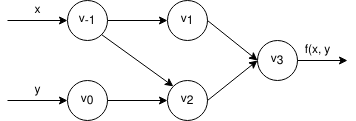
\includegraphics[scale=0.6]{assets/function_trace.png}
  \caption{Computational graph of $f(x, y) = x^2 + (x - y)$}
  \label{fig:func_trace}
\end{figure}

\begin{figure}[h]
  \begin{center}
    \begin{tabular}{ l l l l l | l l l l l }
      \hline
      \multicolumn{5}{l}{Primal trace} & \multicolumn{5}{l}{Tangent trace} \\
      \hline
$v_{-1} $&$=$&$x$&$=$&$2$             &$v'_{-1}$&$=$&$x'$&$=$&$1$ \\
$v_0    $&$=$&$y$&$=$&$1$             &$v'_{0}$&$=$&$y'$&$=$&$0$ \\
      \hline
$v_1    $&$=$&$v_{-1}^2$&$=$&$4$      &$v'_{1}$&$=$&$2*v_{-1}$&$=$&$4$ \\
$v_2    $&$=$&$v_{-1} - v_{0}$&$=$&$1$&$v'_{2}$&$=$&$v'_{-1}-v'_{0}$&$=$&$1$ \\
$v_3    $&$=$&$v_1 + v_2$&$=$&$5$     &$v'_{3}$&$=$&$v'_1 + v'_2$&$=$&$5$ \\
      \hline
$f      $&$=$&$v_3$&$=$&$5$           &$f'$&$=$&$v'_3$&$=$&$5$ \\
      \hline
    \end{tabular}
  \end{center}
  \caption{Primal and tangent traces of $f(x, y) = x^2 + (x - y)$}
  \label{table:func_trace}
\end{figure}

\todo{Fill in}

\subsection{Denotational semantics}
% A formal semantics of programming language: An introduction

The notion of denotational semantics tries to find underlying mathematical models able to underpin the concepts known in programming languages. The most well-known example is the solution given by Dana Scott and Christopher Strachey\cite{Scott1977} for lambda calculi, also called domain theory.
To be able to formalize non-termination and partiality, they thought to use concepts such as partial orderings and least fixed points\cite{aaby2020}.
In this model, programs are interpreted as partial functions and computations as taking the fixpoint of such functions.
Non-termination, on the other hand, is formalized as a value \<bottom> that is lower in the ordering relation than any other element.

In our specific case, we try to find a satisfactory model we can use to show that our implementation of forward mode automatic differentiation is correct when applied to a simply typed lambda calculus.
In the original pen and paper proof of automatic differentiation this thesis is based on, the mathematical models used were diffeological spaces, which are generalization of smooth manifolds.
For the purpose of this thesis, however, this was deemed excessive and much too difficult and time consuming to implement in a mathematically sound manner in \<Coq>.
As such, we chose to make use of \<Coq>'s existing types as denotations and base the relation on the denotations instead of the syntactic structures.
Due to the relative simplicity of the language, we did not yet require domain theoretical concepts. If recursion or iteration were to be added to the language, it is currently expected that these would be needed.

\todo{Fill in}

\subsection{Coq}

\<Coq> is a proof assistant based on the calculus of constructions type theory created by Thierry Coquand and G\'{e}rard Huet\cite{Coquand1988}.
In the 30 years since it has been released, research has contributed to extending the proof assistant with additional features such as inductive and co-inductive data types\cite{Coquand1990}, dependent pattern matching\cite{Sozeau2010} and advanced modular constructions for organizing large mathematical proofs\cite{Sozeau2008}\cite{Mahboubi2013}.

The core of this type theory is based on constructive logic and so many of the laws known in classical logic are not provable.
Examples include the law of the excluded middle, $\forall A, A \vee \neg A$, or the law of functional extensionality, $(\forall x, f(x) = g(x)) \rightarrow f = g$.
In some cases they can, however, be safely added to \<Coq> without making its logic inconsistent.
Due to its usefulness in proving propositions over functions, we will make use of the functional extensionality axiom in \<Coq>.

\subsubsection{Language representation}
\label{sec:language_repr}

\begin{figure}
  \begin{mathpar}
    \inferrule*[Right=\textsc{TVar}]
      {elem\ n\ \Gamma = \tau}
      {\Gamma \vdash var\ n : \tau} \and
    \inferrule*[Right=\textsc{TAbs}]
      {(\sigma, \Gamma) \vdash t : \tau}
      {\Gamma \vdash t : \sigma \rightarrow \tau} \\ \and
    \inferrule*[Right=\textsc{TApp}]
      {\Gamma \vdash t1 : \sigma \rightarrow \tau \\
        \Gamma \vdash t2 : \sigma}
      {\Gamma \vdash t1\ t2 : \tau}
  \end{mathpar}
  \label{fig:stlc_infer}
  \caption{Type-inferrence rules for a simply typed lambda calculus using De-Bruijn indices}
\end{figure}

When defining a simply typed lambda calculus, there are two main possibilities\cite{plfa2019}.
The arguably simpler variant, known as an extrinsic representation, is traditionally the one introduced to new students learning \<Coq>.
In the extrinsic representation, the terms themselves are untyped and typing judgments are defined separately as relations between the types and terms. A basic example of working with this is given in Software Foundations\cite{Pierce:SF2}.
This, however, required many additional lemmas and machinery to be proved to be able to work with both substitutions and contexts as these are defined separate from the terms.
As an example, the preservation property which states that reduction does not change the type of a term, needs to be proven explicitly.
The other approach, also called an intrinsic representation, makes use of just a single well-typed definition.
Ill-typed terms are made impossible by the type checker.
This representation, while beneficial in the proof load, however complicates much of the normal machinery involved in programming language theory.
One example is how one would define operations such as substitutions or weakening.

But even when choosing an intrinsic representation, the problem of variable binding persists.
Much meta-theoretical research has been done on possible approaches to this problem each with their own advantages and disadvantages.
The POPLmark challenge gives a comprehensive overview of each of the possibilities in various proof assistants\cite{Aydemir2005}.
An example of an approach is the nominal representation where every variable is named.
While this does follow the standard format used in regular mathematics, problems such as alpha-conversion and capture-avoidance arise.

\begin{listing}[h]
  \begin{minted}{coq}
  Inductive ty : Type :=
    | ~unit~ : ~ty~
    | ~\Rightarrow~ : ~ty \rightarrow ty \rightarrow ty~.

  Inductive tm : Type :=
    | var : ~string \rightarrow tm ~
    | abs : ~string \rightarrow ty \rightarrow tm \rightarrow tm~
    | app : ~tm \rightarrow tm \rightarrow tm~.
  \end{minted}
  \caption{Simply typed \lambda-calculus using an extrinsic nominal representation.}
  \label{lst:nominal_stlc}
\end{listing}

The approach used in the rest of this thesis is an extension of the De-Bruijn representation which numbers variables relative to the binding lambda term.
In this representation the variables are referred to as well-typed De-Bruijn indices.
A significant benefit of this representation is that the problems of capture avoidance and alpha equivalence are avoided.
As an alternative, instead of using numbers to represent the distance, indices within the typing context can be used to ensure that a variable is always well-typed and well-scoped.
While the idea of using type indexed terms has been both described and used by many authors\cite{Altenkirch99}\cite{McBride04}\cite{Adams06}, the specific formulation used in this thesis using both substitutions and rename operations was fleshed out in Coq by Nick Benton, et. al.\cite{Benton2011}, and was also used as one of the examples in the second POPLmark challenge which deals with logical relations\cite{poplmark_reloaded}.
While this does avoid the problems present in the nominal representation, it unfortunately does have some problems of its own.
Variable substitutions have to be defined using two separate renaming and substitution operations.
Renaming is formulated as extending the typing context of variables, while substitution actually swaps the variables for terms.
Due to using indices from the context as variables, some lifting boilerplate is also needed to manipulate contexts.

\begin{listing}[h]
  \begin{minted}{coq}
  Inductive ~\tau \in \Gamma~ : Type :=
    | Top : ~\forall \Gamma \tau, \tau \in (\tau::\Gamma)~
    | Pop : ~\forall \Gamma \tau \sigma, \tau \in \Gamma \rightarrow \tau \in (\sigma::\Gamma)~.

  Inductive tm ~\Gamma \tau~ : Type :=
    | var : ~\forall \Gamma \tau, \tau \in \Gamma \rightarrow tm \Gamma \tau~
    | abs : ~\forall \Gamma \tau \sigma, tm (\sigma::\Gamma) \tau \rightarrow tm \Gamma (\sigma \Rightarrow \tau)~
    | app : ~\forall \Gamma \tau \sigma, tm \Gamma (\sigma \Rightarrow \tau) \rightarrow tm \Gamma \sigma \rightarrow tm \Gamma \tau~.
  \end{minted}
  \caption{Basis of a simply typed \lambda-calculus using a strongly typed intrinsic formulation.}
  \label{lst:strong_stlc}
\end{listing}
\todo{Extend example}

\subsubsection{Dependently-typed programming in Coq}

In \<Coq>, one can normally write function definitions using either case-analysis as is done in other functional languages, or using \<Coq>'s tactics.
If proof terms are present in the function definition, however, it is customary to write it using tactics because of the otherwise complicated and verbose code due to the previously poor support for dependent pattern matching in Coq.
But if the functionality is not immediately apparent from the function signature, it can be hard to recognize what the function then computes.
One other possibility would be to write the function as a relation between its input and output.
This also has its limitations as you then lose computability as Coq treats these definitions opaquely. In this case the standard \<simpl> tactic which invokes \<Coq>'s reduction mechanism is not able to reduce instances of the term.
This often requires the user to write to write many more proofs to be able to work with the definitions.

As an example, we will work through defining a length indexed list and a corresponding head function, which is well known to be partial.
Using the \<Coq> keyword return, it is possible to let the return type of a match expression depend on the result of one of the type arguments.
This makes it possible to specify what the return type of the empty list should be.
In snippet~\ref{lst:dt_ilist}, we use the unit type which contains just one inhabitant, \<tt>.

\begin{listing}
  \begin{minted}{coq}
  Inductive ilist : ~Type \rightarrow nat \rightarrow Type~ :=
    | nil : ~\forall A, ilist A 0~
    | cons : ~\forall A n, A \rightarrow ilist A n \rightarrow ilist A (S n)~

  Definition hd {A} n (ls : ilist A n) :=
    match ls in (ilist A n) return
      (match n with
      | O => unit
      | S _ => A end) with
    | nil => tt
    | cons h _ => h
  end.
  \end{minted}
  \caption{Definition of a length indexed list and hd using the return keyword, adapted from Certified Programming with Dependent Types\cite{ChlipalaCPDT}.}
  \label{lst:dt_ilist}
\end{listing}

Mathieu Sozeau introduces an extension to \<Coq> via a new keyword \<Program> which allows the use of case-analysis in more complex definitions\cite{Sozeau2006}\cite{Sozeau2007}.
To be more specific, it allows definitions to be specified separately from its accompanying proofs, possibly filling them in automatically if possible.
While this does improve on the previous situation, using the definitions in proofs can often be unwieldy due to the amount of boilerplate introduced.
This makes debugging error messages even harder than it already is in a proof assistant. This approach was used by Benton in his formulation of strongly typed terms.

Sozeau further improves on this introducing a method for user-friendlier dependently-typed pattern matching in \<Coq> in the form of the \<Equations> library\cite{Sozeau2010}\cite{Sozeau2019}.
This introduces \<Agda>-like dependent pattern matching with with-clauses.
It does this by using a notion called coverings, where a covering is a set of equations such that the pattern matchings of the type signature are exhaustive.
There are two main ways to integrate this in a dependently typed environment, externally where it is integrated as high-level constructs in the pattern matching core as \<Agda> does it, or internally by using the existing type theory and finding witnesses of the covering to prove the definition correct, which is the approach used by Sozeau.
Due to the intrinsic typeful representation this paper uses, much of this was invaluable when defining the substitution operators as the regular type checker in Coq often had difficulty type checking dependently typed terms in certain cases.

\begin{listing}
  \begin{minted}{coq}
  Equations hd {A n} (ls : ilist A n) (pf : n <> 0%nat) : A :=
  hd nil pf with pf eq_refl := {};
  hd (cons h n) _ := h.
  \end{minted}
  \caption{Definition of hd using \<Equations>}
  \label{lst:dt_ilist_hd_equations}
\end{listing}

\todo{Fill in}

\subsection{Logical relations}

Logical relations is technique often employed when proving programming language properties of statically typed languages\cite{skorstengaard2019introduction}. There are two main ways they are used, namely as unary and binary relations.
Unary logical relations, also known as logical predicates, are predicates over single terms and are typically used to prove language characteristics such as type safety or strong normalization.
Binary logical relations on the other hand are used to prove program equivalences, usually in the context of denotational semantics as we will do.
Logical relations in essence are simply relations between terms defined by induction on the types. A logical relations proof consists of 2 steps.
The first usually states that well-typed terms are in the relation, while the second states that the property of interest follows from the relation.
The second step is easier to prove as it usually follows from the definition of the relation. The first on the other hand, will often require proving a generalized variant, called the fundamental property of the logical relation.
In most cases this requires that the relation is correct with respect to applying substitutions.

A well-known logical relations proof is the proof of strong normalization of well-typed terms, which states that all well-typed terms are either terminal values or can be reduced further.
An example of a logical relation used in such a proof using the intrinsic strongly-typed formulation is given in snippet~\ref{lst:sn_logical_relation}.
Noteworthy is the case for function types, which indicates that application should maintain the strongly normalization relation.
The proof given in the paper this thesis is based on, is a logical relations proof on the denotation semantics using diffeological spaces as its domains\cite{huot2020correctness}.
A similar, independent proof of correctness was given by Barthe, et. al.\cite{barthe2020versatility} using an syntactic relation.

\begin{listing}
  \begin{minted}{coq}
    Equations SN {~\Gamma~} ~\tau~ (t : ~tm \Gamma \tau~): Prop :=
    SN unit t := halts t;
    SN ~(\tau \Rightarrow \sigma)~ t := halts t ~$\wedge$~
      ~(\forall (s : tm \Gamma \tau), SN \tau s \rightarrow SN \sigma (app \Gamma \sigma \tau t s))~;
  \end{minted}
  \caption{Example of a logical predicate used in a strong normalizations proof in the intrinsic strongly-typed formulation}
  \label{lst:sn_logical_relation}
\end{listing}

\section{Preliminary Results}

\subsection{Language definitions}

We currently mimic the base types used in the paper~\cite{huot2020correctness} extended with sum types, shown in snippet~\ref{lst:stlc_types}.
The paper itself initially makes use of the standard types found in a simply typed lambda calculus extended with products and R as the only ground type.
These are also the types used by Barthe, et. al.\cite{barthe2020versatility} in their proof. In a later section Stanton, Huot and \Vakar{} extended their language with sum and inductive types.
Note that we use the unconventional symbol \texttt{<+>} for sum types instead of the more common \texttt{+}, because Coq already uses the latter for their own sum types.

\begin{listing}
  \begin{minted}{coq}
  Inductive ty : Type :=
    | Real : ty
    | ~\Rightarrow~ : ~ty \rightarrow ty \rightarrow ty~
    | ~\times~ : ~ty \rightarrow ty \rightarrow ty~
    | ~<+>~ : ~ty \rightarrow ty \rightarrow ty~.
  \end{minted}
  \caption{Definition of the types present in the language}
  \label{lst:stlc_types}
\end{listing}

We have chosen the intrinsic strongly-typed formulation used in \cite{Benton2011} as the general framework to work in.
This includes the various substitution and lifting operations for working with typing contexts. Typing contexts themselves consists of lists of types, while variables are typed indices into this list. We almost perfectly mimic the example shown in snippet~\ref{lst:strong_stlc}.

We have simplified a few of the language constructs used in \cite{huot2020correctness}, shown in snippet~\ref{lst:stlc_terms}. For working with product types they make use of n-products and pattern matching, while we have opted for projection tuples. They proceeded to extended their base language with arbitrarily sized variant types, which we have substituted for standard sums reminiscent of the \<Either> type in Haskell along with specialized case expressions. Both of these changes were intended to simplify the language as much as possible while still retaining the same core functionality and types.

\begin{listing}
  \begin{minted}{coq}
Definition Ctx {x} : Type := list x.

Inductive tm ~(\Gamma : Ctx) : ty \rightarrow Type~ :=
  (* Base STLC *)
  | var : ~forall \tau,
    \tau ∈ \Gamma \rightarrow tm \Gamma \tau~
  | app : ~forall \tau \sigma,
    tm \Gamma (\sigma \Rightarrow \tau) \rightarrow
    tm \Gamma \sigma \rightarrow
    tm \Gamma \tau~
  | abs : ~forall \tau \sigma,
    tm (\sigma::\Gamma) \tau \rightarrow tm \Gamma (\sigma \Rightarrow \tau)~

  (* Operations on the real numbers *)
  | const : ~R \rightarrow tm \Gamma Real~
  | add : ~tm \Gamma Real \rightarrow tm \Gamma Real \rightarrow tm \Gamma Real~

  (* Projection products *)
  | tuple : ~forall {\tau \sigma},
    tm \Gamma \tau \rightarrow
    tm \Gamma \sigma \rightarrow
    tm \Gamma (\tau \times \sigma)~
  | first : ~forall {\tau \sigma}, tm \Gamma (\tau \times \sigma) \rightarrow tm \Gamma \tau~
  | second : ~forall {\tau \sigma}, tm \Gamma (\tau \times \sigma) \rightarrow tm \Gamma \sigma~

  (* Sums *)
  | case : ~forall {\tau \sigma \rho}, tm \Gamma (\tau + \sigma) \rightarrow
    tm \Gamma (\tau \Rightarrow \rho) \rightarrow
    tm \Gamma (\sigma \Rightarrow \rho) \rightarrow
    tm \Gamma \rho~
  | inl : ~forall \tau \sigma, tm \Gamma \tau \rightarrow tm \Gamma (\tau + \sigma)~
  | inr : ~forall \tau \sigma, tm \Gamma \sigma \rightarrow tm \Gamma (\tau + \sigma).~

  \end{minted}
  \caption{Definition of the language constructs present in the language}
  \label{lst:stlc_terms}
\end{listing}

\subsection{Preliminary proofs}

We have completed a preliminary proof of \texttt{Theorem 1} of \cite{huot2020correctness}. This consists of a formulation of semantic correctness of a forward-mode automatic differentiation algorithm using a macro. The proof is done using a logical relation on the denotational semantics using \<Coq>'s types as the underlying domain. The definition of the logical relation along with the lemma stating its fundamental property is shown in snippet~\ref{lst:direct_logical_relation} and~\ref{lst:direct_fundamental}, while snippet~ \ref{lst:direct_correctness} states the actual correctness theorem.

\begin{listing}
  \begin{minted}{coq}
Equations S ~\tau~ :
  ~(R \rightarrow $\llbracket$ \tau $\rrbracket$) \rightarrow (R \rightarrow $\llbracket$ D \tau $\rrbracket$) \rightarrow Prop~ :=
S Real f g :=
  ~(\forall (x : R), ex\_derive f x) $\wedge$~
  (fun r => g r) =
    (fun r => (f r, Derive f r));
S (~\sigma \times \rho~) f g :=
  ~\exists~ f1 f2 g1 g2,
  ~\exists (s1 : S \sigma f1 f2) (s2 : S \rho g1 g2),~
    (f = fun r => (f1 r, g1 r)) ~$\wedge$~
    (g = fun r => (f2 r, g2 r));
S (~\sigma \Rightarrow \rho~) f g :=
  ~\forall (g1 : R \rightarrow $\llbracket$ \sigma $\rrbracket$),~
  ~\forall (g2 : R \rightarrow $\llbracket$ D \sigma $\rrbracket$),~
    ~S \sigma g1 g2 \rightarrow~
    ~S \rho (fun x => f x (g1 x))~
      (fun x => g x (g2 x));
S (~\sigma <+> \rho~) f g :=
  (~\exists~ g1 g2,
    ~S \sigma g1 g2 $\wedge$~
      ~f = inl \circ g1 $\wedge$~
      ~g = inl \circ g2) $\vee$~
  (~\exists~ g1 g2,
    ~S \rho g1 g2 $\wedge$~
      ~f = inr \circ g1 $\wedge$~
      ~g = inr \circ g2)~.
  \end{minted}
  \caption{Definition of the logical relation}
  \label{lst:direct_logical_relation}
\end{listing}

\begin{listing}
  \begin{minted}{coq}
Inductive instantiation : ~forall \Gamma~,
    ~(R \rightarrow $\llbracket$ \Gamma $\rrbracket$) \rightarrow (R \rightarrow $\llbracket$ D \Gamma $\rrbracket$) \rightarrow Prop :=~
| inst_empty : instantiation [] (const tt) (const tt)
| inst_cons :
  ~\forall \Gamma \tau g1 g2,~
  ~\forall (sb: R \rightarrow $\llbracket$ \Gamma $\rrbracket$) (Dsb: R \rightarrow $\llbracket$ D \Gamma $\rrbracket$),~
    ~instantiation \Gamma sb Dsb \rightarrow~
    ~S \tau g1 g2 \rightarrow~
    ~instantiation (\tau::\Gamma)
      (fun r => (g1 r, sb r)) (fun r => (g2 r, Dsb r)).~

Lemma fundamental :
    ~\forall \Gamma \tau (t : tm \Gamma \tau),~
    ~\forall (sb : R \rightarrow $\llbracket$ \Gamma $\rrbracket$) (Dsb : R \rightarrow $\llbracket$ D \Gamma $\rrbracket$),~
  ~instantiation \Gamma sb Dsb \rightarrow~
  ~S \tau ($\llbracket$ t $\rrbracket$ \circ sb)~
    ~($\llbracket$ Dtm t $\rrbracket$ \circ Dsb).~
  \end{minted}
  \caption{Definition of the fundamental property of the logical relation in snippet~\ref{lst:direct_logical_relation}}
  \label{lst:direct_fundamental}
\end{listing}

\begin{listing}
  \begin{minted}{coq}
Equations D n
  ~(f : R \rightarrow $\llbracket$ repeat Real n $\rrbracket$): R \rightarrow $\llbracket$ map Dt (repeat Real n) $\rrbracket$ :=~
D 0 f r := f r;
D (S n) f r :=
  ~(((fst \circ f) r, Derive (fst \circ f) r), D n (snd \circ f) r).~

Inductive differentiable : ~\forall n, (R \rightarrow $\llbracket$ repeat Real n $\rrbracket$) \rightarrow Prop :=~
| differentiable_0 : differentiable 0 (fun _ => tt)
| differentiable_Sn :
  ~\forall n (f : R \rightarrow $\llbracket$ repeat Real n $\rrbracket$),~
  ~\forall (g : R \rightarrow R),~
    ~differentiable n f \rightarrow~
    ~(\forall x,~ ex_derive g x) ~\rightarrow~
    ~differentiable (S n) (fun x => (g x, f x)).~

Theorem semantic_correct_R :
  ~\forall n (t : tm (repeat Real n) Real),~
  ~\forall (f : R \rightarrow $\llbracket$ repeat Real n $\rrbracket$),~
    ~differentiable n f \rightarrow~
    ~($\llbracket$ Dtm t $\rrbracket$ \circ D n f) =~
      ~fun r => ($\llbracket$ t $\rrbracket$ (f r),~
        ~Derive (fun (x : R) => $\llbracket$ t $\rrbracket$ (f x)) r).~
  \end{minted}
  \caption{Definition of the correctness theorem}
  \label{lst:direct_correctness}
\end{listing}

\section{Timetable and Planning}

\subsection{Extensions}

We will be looking to extend the current prototype proof with the continuation-based AD macro mentioned in \cite{huot2020correctness}.
We will also try to extend the proof with a small imperative language we are able to translate into the simply typed lambda calculus.
The goal is to work towards results usable in the context of program optimizations.
One possibility is to go towards a SSA (static single assignment) representation which has many benefits as a well-known possible internal representation for use in compilers\cite{Pop2006}.
One other benefit is that this representation can also be transformed into a minimal functional language\cite{chakravarty2004347}.

\todo{Fill in}

\subsection{Deadlines}

The hard deadlines for the first and second phases of the thesis are respectively May $1^{st}$ and September $18^{th}$. The ambition is to follow the following framework of deadlines. Note that until the proofs deadline, the proofs and paper will largely be written in parallel with each other.

\todo{Fill in}

\begin{center}
  \begin{tabular}{ | m{5cm} | m{5cm} | }
    \hline
    Deadline          & Date  \\
    \hline
    Proposal deadline & 1/5/2020 \\
    Finish proofs & 15/7/2020 \\
    Finish first draft & 15/8/2020 \\
    Thesis deadline & 18/9/2020 \\
    \hline
  \end{tabular}
\end{center}

\printbibliography
\makeatother
\end{document}